\documentclass[12pt]{article}
\usepackage{amsmath, amssymb, amsfonts, geometry, pgfplots, graphicx}

\usepackage{listings}
\usepackage{xcolor} % Optional: for customizing colors

\lstset{
  language=Python,
  backgroundcolor=\color{lightgray},   % Background color for code
  basicstyle=\ttfamily\footnotesize,    % Font style and size
  keywordstyle=\color{blue},            % Color of keywords
  commentstyle=\color{green},           % Color of comments
  stringstyle=\color{red},              % Color of strings
  numbers=left,                         % Line numbers on the left
  numberstyle=\tiny\color{gray},        % Style for line numbers
  stepnumber=1,                         % Step between line numbers
  numbersep=5pt,                        % Distance from code to line numbers
  frame=single,                         % Add a frame around the code
  tabsize=4,                            % Number of spaces per tab
  captionpos=b,                         % Position of the caption (b for bottom)
}
\pgfplotsset{compat=1.18}

% Page Setup
\geometry{top=1in, bottom=1in, left=1in, right=1in}

\title{Mat104 Oblig3}
\author{Thobias Høivik, Gunnar Salbu, Birk Tangen, \\  
Holly Storøy, Knut Rokne, Glenn Boine}
\date{March 3 2025}

\begin{document}

\maketitle
\section*{Oppgave 1}
\(f(x) = \sqrt{x+4}, \quad D_f = [-4, 0] \).
\subsection*{a) }
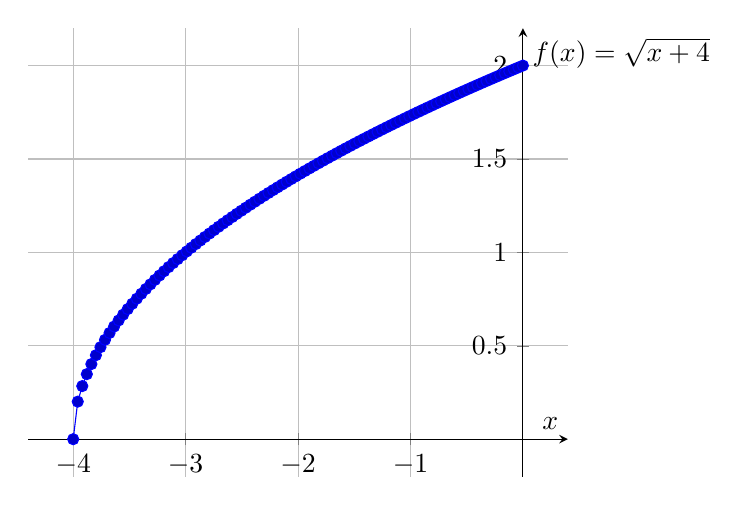
\begin{tikzpicture}
    \begin{axis}[
        axis lines = middle,
        xlabel = $x$,
        ylabel = {$f(x) = \sqrt{x + 4}$},
        domain=-4:0,
        samples=100,
        enlargelimits,
        grid=both 
    ]
        \addplot {sqrt(x + 4)};
    \end{axis}
\end{tikzpicture}

\subsection*{b)}
Vi begynner med å finne
\[
\frac{d}{dx}f(0) = [\frac{1}{2\sqrt{x + 4}}]_{x=0}
= \frac{1}{4}
\]

\noindent
Tangentlinjen vil være gitt ved \(y-y_0 = m(x-x_0)\)
\[
  y-2 = \frac{1}{4}(x-0) \Leftrightarrow y-2 = \frac{1}{4}x 
  \Leftrightarrow \boxed{y=\frac{1}{4}x + 2}
\]

\subsection*{c)}
\(\sqrt{3.96} = \sqrt{-0.04 + 4} = f(-0.04) \approx f(0), 
\quad \therefore \sqrt{4} \approx [m(x-x0) - y_0]_{x = 0.04} 
= -\frac{0.04}{4} + 2 = \boxed{1.99}\)

\subsection*{d)}
Først må vi finne linjen som går parallellt gjennom \((-4, 0) \land (0, 2)\).
\begin{gather*}
  y = mx + b \\ 
  \Delta x = 4, \quad \Delta y = 2 \\ 
  m = \frac{\Delta y}{\Delta x} = \frac{2}{4} = \frac{1}{2} \\ 
  b = 2 \because y = 0 \Leftrightarrow x = -4 \\ 
  y = \frac{1}{2}x + 2 \\ 
\end{gather*}
For å finne en tangentlinje parallell med denne, må vi løse 
\[
f'(x_0) = \frac{1}{2}.
\]
Løser \( \frac{1}{2\sqrt{x_0+4}} = \frac{1}{2} \):
\begin{gather*}
    \sqrt{x_0+4} = 1 \quad \Rightarrow \quad x_0 + 4 = 1 
    \\ \Rightarrow \quad \boxed{x_0 = -3}
\end{gather*}
Beregner \( y_0 \):
\[
    \boxed{y_0 = f(-3) = \sqrt{-3+4} = 1}
\]
Tangentlinjen er:
\[
y - 1 = \frac{1}{2}(x + 3)
\]
Omskriving gir:
\[
\boxed{y = \frac{x}{2} + \frac{5}{2}}
\]

\break
\section*{Oppgave 2}
\subsection*{a)}
\begin{gather*}
  \lim_{x\to0} \frac{3^x-e^x}{\pi^x-\cos{2x}} \\ 
  x = 0 \rightarrow \frac{0}{0} \\ 
  \lim_{x\to0} \frac{3^x-e^x}{\pi^x-\cos{2x}}
  = \lim_{x\to0}\frac{\frac{d}{dx}|_{x=0} \quad 3^x - e^x}
  {\frac{d}{dx}|_{x=0} \quad \pi^x - \cos{2x}}
  \\ 
  = \frac{[\ln(3) \times 3^x - e^x]_{x=0}}{[\ln(\pi) \times \pi^x + 2\sin(2x)]_{x=0}}
  = \frac{\ln(3) - 1}{\ln(\pi) + 2 \times 0} 
  = \boxed{\frac{\ln(\frac{3}{e})}{\ln(\pi)}}
\end{gather*}

\subsection*{b)}
\begin{gather*}
  \lim_{x\to1} \frac{\ln x}{x^2-1} \\ 
  x = 1 \rightarrow \frac{0}{0} \\ 
  \lim_{x\to1} \frac{\ln x}{x^2-1} = \lim_{x\to1} \frac{1}{x} \div 2x 
  = \boxed{\frac{1}{2}} \\ 
\end{gather*}

\subsection*{c)}
\begin{gather*}
  \lim_{x\to\infty } \frac{x^2}{e^x+x^2} \\ 
  \text{Husk at } (e^x)' = e^x \text{, og mer presist at } 
  \frac{d^n}{dx^n} e^x = e^x, \quad \forall n \in \mathbb Z \\ 
  \text{Observer da at vi kan derivere } x^2 
  \text{ to ganger oppe og nede for oppnå svaret.} \\
  \lim_{x\to\infty}\frac{2}{e^x+2} = \boxed{0} \\ 
  e^x \text{ går mot uendelig så uttrykket går mot 0} \\
  \text{Viss vi ikke ville brukt l'Hopital kunne vi tatt } \div x^2 
  \\ \text{ oppe og nede 
  og så eventuellt argumentert at } x^2 < e^x, \quad \forall x \geq 0 
\end{gather*}

\break
\section*{Oppgave 3}
\subsection*{a)}
\begin{gather*}
  \displaystyle\int_{0}^{4}3x^2-1 dx = [x^3-x]_{x=0}^4 = 4^3 - 4 = 64-4 = 60
\end{gather*}

\subsection*{b)}
\begin{gather*}
  \displaystyle\int \sin(2x) dx \\ 
  \text{La } u = 2x \Rightarrow \quad du = 2dx \Leftrightarrow \frac{du}{2} = dx \\ 
  \displaystyle\int \sin(2x) dx = \frac{1}{2} \displaystyle\int \sin(u) du \\
  = \frac{1}{2} (-\cos(u)) + c = \boxed{-\frac{1}{2} \cos(2x) + C}
\end{gather*}

\subsection*{c)}
\begin{gather*}
  I = \displaystyle\int xe^{x^2 + 1} dx \\ 
  \text{La } u = x^2 + 1 \Rightarrow \frac{du}{2} = dx \\ 
  I = \frac{1}{2}\displaystyle\int e^u du
  = \frac{1}{2} e^u + C = \boxed{\frac{1}{2} e^{x^2+1} + C}
\end{gather*}

\break
\section*{Oppgave 4}
\[I = \displaystyle\int_{0}^{\frac{\pi}{4}} 4 + 2x \tan (x) dx\]
\subsection*{a)}
Vi deler intervalet \([0, \frac{\pi}{4}]\) i 4. 
Lengden av hver delinterval er da 
\[ 
  h = \frac{\frac{\pi}{4} - 0}{4} = \frac{\pi}{16} 
\]
Punktene i oppdelingen blir 
\begin{gather*} 
  x_0 = 0 \\
  x_1 = \frac{\pi}{16} \\
  x_2 = \frac{2\pi}{16} = \frac{\pi}{8} \\
  x_3 = \frac{3\pi}{16} \\ 
  x_4 = \frac{4\pi}{16} = \frac{\pi}{4}
\end{gather*}

\subsection*{b)}
La \(X = \{x_0, x_1, x_2, x_3, x_4\}\). Vi kan da tilnærme integralet 
\begin{gather*}
  \displaystyle\int_{a}^{b}f(x)dx \approx 
  \frac{h}{2} [f(x_0) 
  + 2(\displaystyle\sum_{i = 1}^{|X| - 1} f(x_i)) +
  f(x_4) ] \\ 
  \boxed{A \approx \frac{\pi}{32}[4+2f(x_1)+2f(x_2)+2f(x_3)+x_4] \approx 3.5}
\end{gather*}

\break
\subsection*{c)}
Ved å tilnærme med \(n=25\) får vi 3.5135845378158312 som er lik geogebra sin 
tilnærming til tredje desimalpunkt.

\noindent
\textbf{Kode: }
\begin{lstlisting}[language=Python]
import math

def f(x):
    return 4 + 2 * x * math.tan(x)

def trapezoidal_rule(a, b, n):
    h = (b - a) / n
    result = 0.5 * (f(a) + f(b))  
    for i in range(1, n):
        result += f(a + i * h) 
    result *= h  
    return result

a = 0
b = math.pi / 4
n = 25

integral_value = trapezoidal_rule(a, b, n)

print(f'Estimert verdi: {integral_value}')
\end{lstlisting}

\break 
\section*{Oppgave 5}
\[f(x)=2x^3+9x^2-24x+1\]

\subsection*{a)}
\begin{gather*}
  \frac{df}{dx} = 6x^2+18x-24 \\ 
  6x^2 + 18x - 24 = 0 \quad | \div 6 \\ 
  x^2 + 3x - 4 = 0 \Leftrightarrow (x+4)(x-1) = 0 \Rightarrow x = -4 \land x = 1 \\ 
  x < -4 \text{, f.eks } f'(-5)=36 > 0 \\ 
  x \in (-4,1) \rightarrow f'(0)= -24 < 0 \\ 
  x > 1 \rightarrow f'(2) = 36 > 0 \\ 
  \therefore x \in \mathbb R - (-4,1) \Rightarrow f'(x) > 0 
  \land x \in (-4,1) \Rightarrow f'(x) < 0
\end{gather*}

\subsection*{b)}
Vi har allerede funne \(f'(x) = 0: \quad x = 1 \land x = -4\). For å finne 
ut om de er bunn- eller topp-punkt kan vi ta den andrederiverte.
\begin{gather*} 
  f''(x)=12x + 18 \\ 
  f''(-4) = -30 < 0 \\ 
  f''(1) = 30 > 0
\end{gather*}
Vi har et bunn-punkt ved \(x=1\) og topp-punkt ved \(x = -4\). 
\(f(1) = -12 \land f(-4) = 113\).

\subsection*{c)}
\begin{gather*}
  f''(x) = 12x + 18 = 0 \\
  12x = -18 \quad \Rightarrow \quad x = -\frac{3}{2}
\end{gather*}
Funksjonen skifter krumning ved \( x = -\frac{3}{2} \), så vi har et vendepunkt der. For å avgjøre om funksjonen er konveks eller konkav, ser vi på fortegnet til \( f''(x) \) på intervallene:

- For \( x < -\frac{3}{2} \) (for eksempel \( x = -2 \)):
  \[
  f''(-2) = 12(-2) + 18 = -24 + 18 = -6 < 0
  \]
  Funksjonen er \textbf{konkav} på \( (-\infty, -\frac{3}{2}) \).

- For \( x > -\frac{3}{2} \) (for eksempel \( x = 0 \)):
  \[
  f''(0) = 12(0) + 18 = 18 > 0
  \]
  Funksjonen er \textbf{konveks} på \( (-\frac{3}{2}, \infty) \).

Vendepunktet skjer når \( f''(x) = 0 \), altså ved \( x = -\frac{3}{2} \).
\[
f\left( -\frac{3}{2} \right) = 50.5
\]

Så, vendepunktet er ved \( x = -\frac{3}{2} \) 
og \( f\left( -\frac{3}{2} \right) = 50.5 \).

\subsection*{d)} 
\begin{figure}[h]
    \centering
    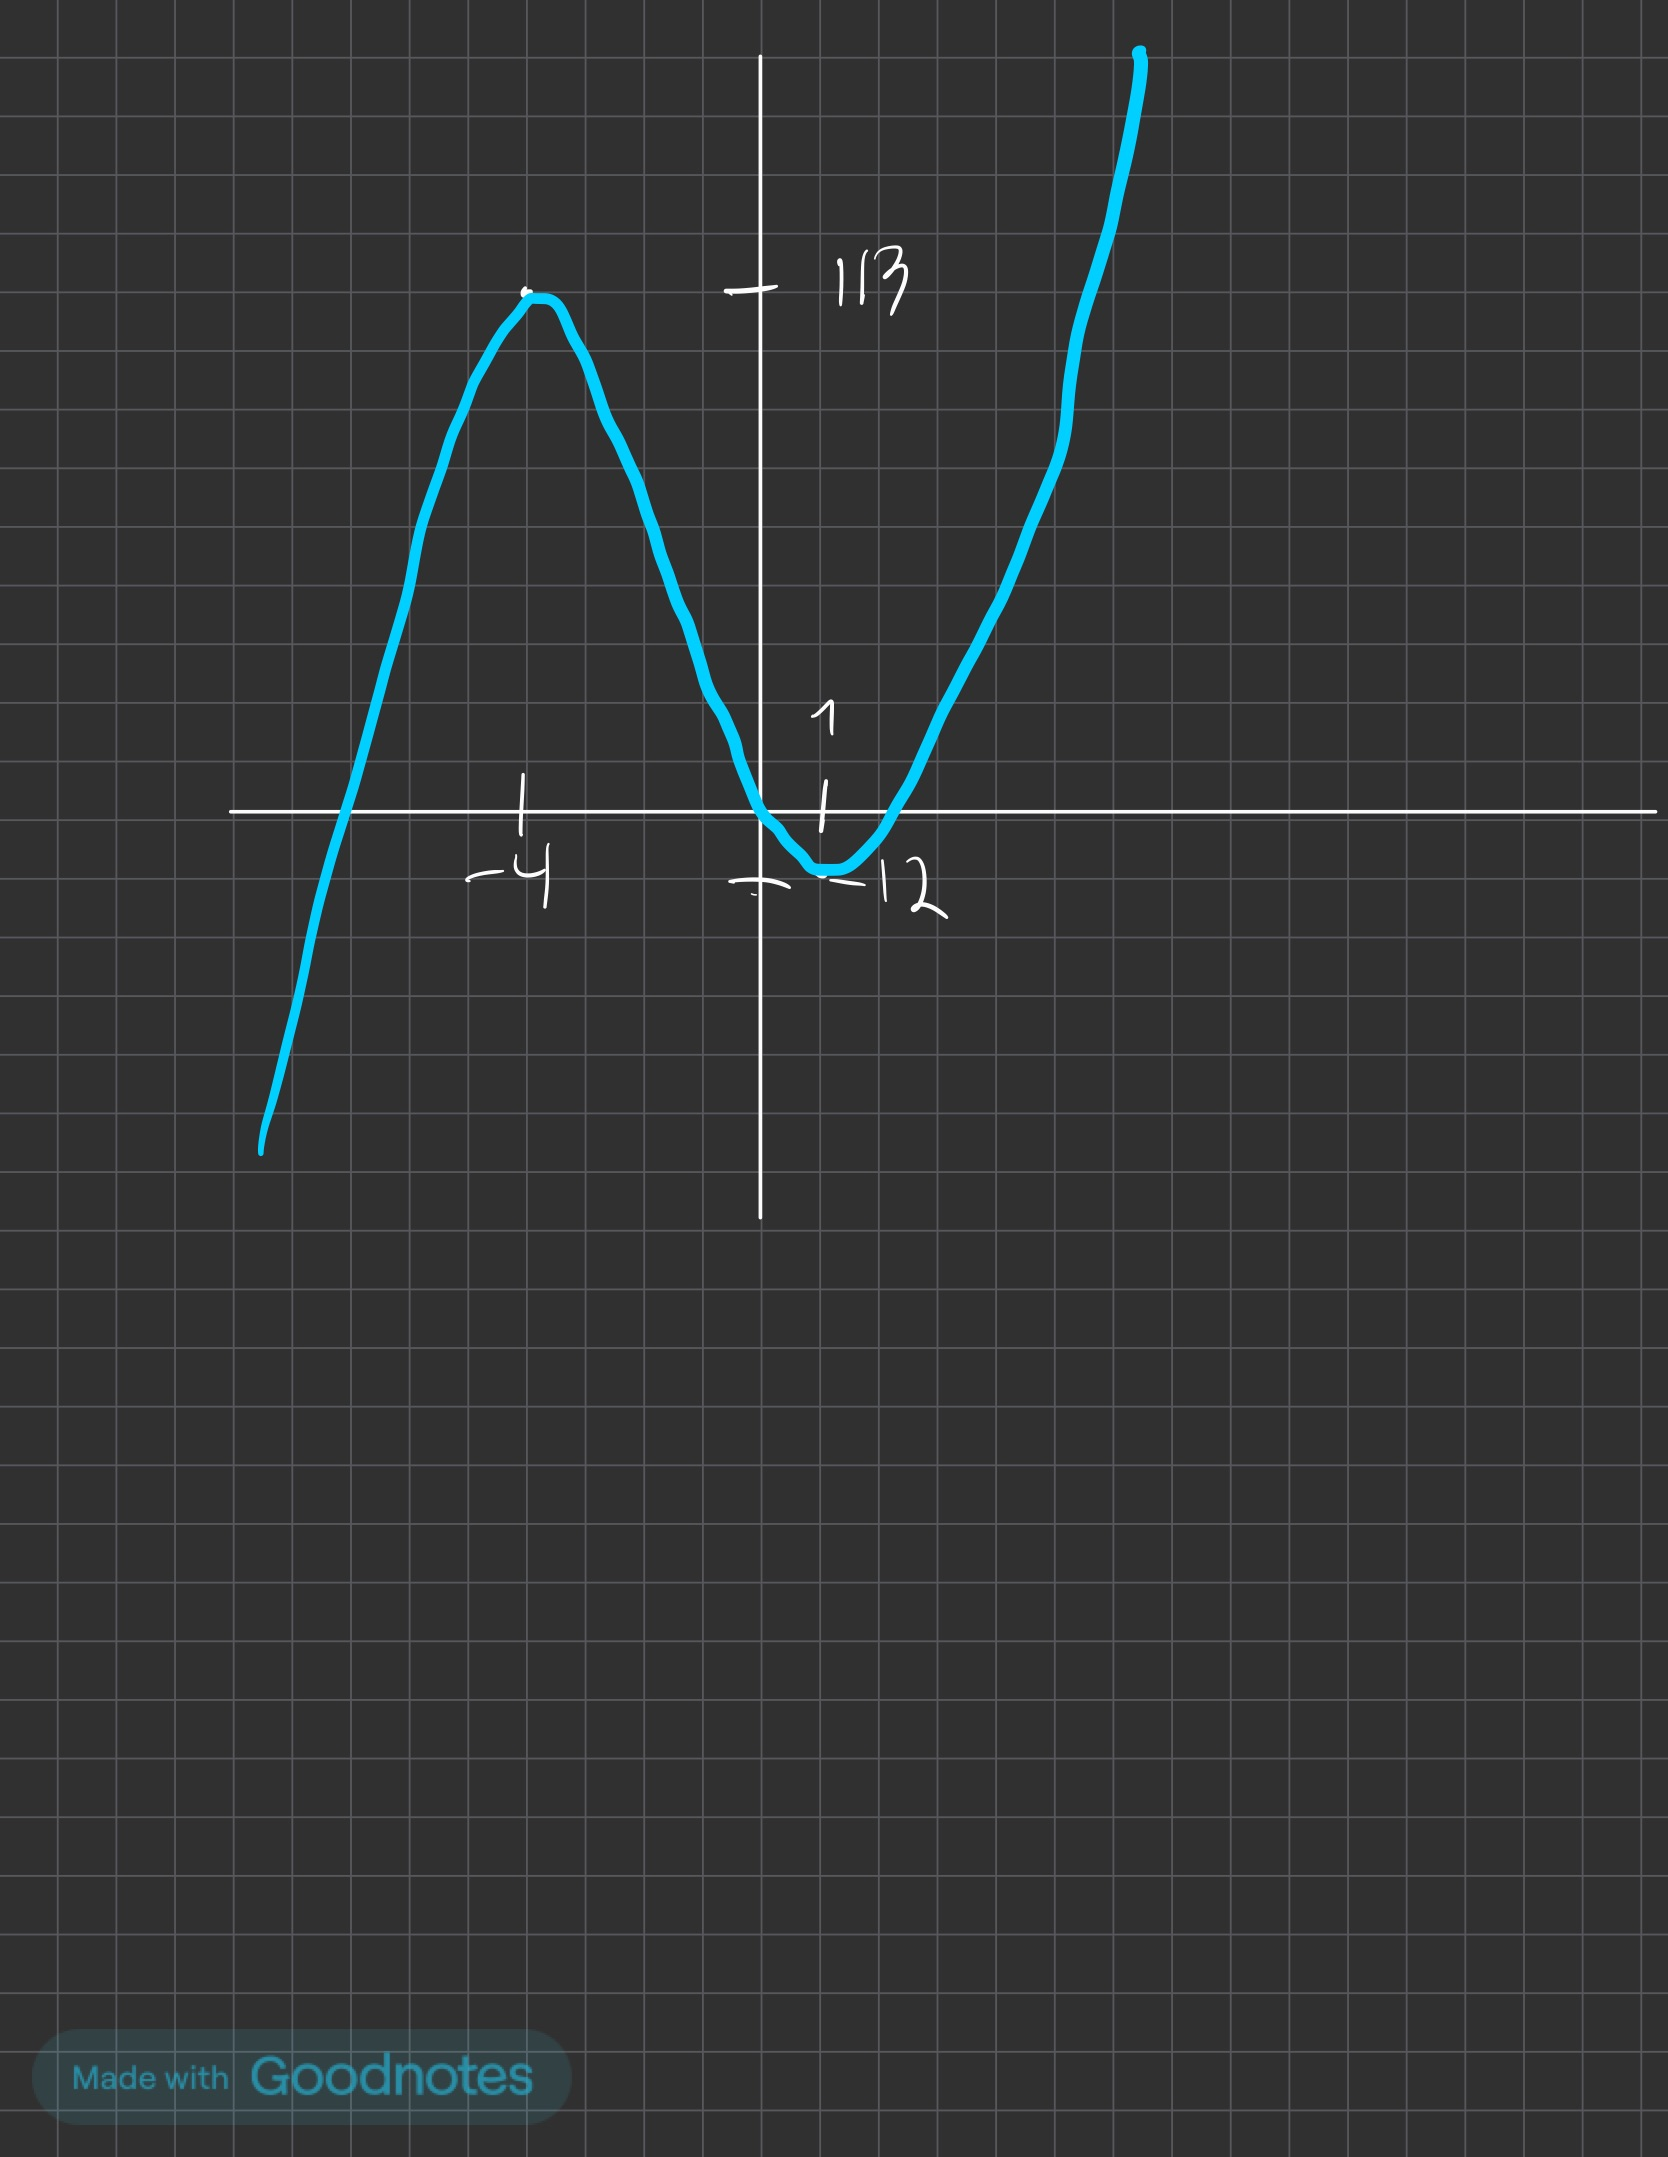
\includegraphics[width=0.7\textwidth]{./MatOblig3.jpg}
    \label{fig:bilde}
\end{figure}

\subsection*{e)}
\[
  f(-8) < 0 \quad f(-4) > 0 \quad f(1) < 0 \quad f(2) > 0
\]
f er kontinuerlig så mellom hver av de 3 parene over må det eksistere alle mulige reelle tal imellom dem, der iblant 0. 

\subsection*{f/g)}
\textbf{Kode: }
\begin{lstlisting}[language=Python]
def f(x):
    return 2*x*x*x + 9*x*x - 24*x + 1

def df(x):
    return 6*x*x + 9*x - 24

xN = 0 
def findZero(xN, f, df, tolerance = 0.000000001):
    xNext = xN - f(xN) / df(xN)
    if (abs(xNext - xN) < tolerance):
        return xNext
    return findZero(xNext, f, df, tolerance)

print(f"Start value for x: {xN}")
print(findZero(xN, f, df))
\end{lstlisting}

\noindent 
Vi velger startpunkt \(s_1 = -5, s_2 = -1, s_3 = 3\) ved hjelp av grafen og det vi 
har lært om funksjonen.

\end{document}
